
\documentclass[12pt,a4paper]{article} 

\usepackage{float,times,graphicx,mathtools}
\usepackage{amsmath}
\usepackage{amsfonts}
\usepackage{amssymb}
\usepackage{latexsym}
\usepackage{epsfig}
\usepackage{graphicx}
\usepackage{caption}
\usepackage{subcaption}
\usepackage{color}
\usepackage{pdfpages}
\usepackage{natbib}
\usepackage[space]{grffile}
\usepackage{wrapfig}
\usepackage{subcaption}
\usepackage{url}
\usepackage{bbm}
\usepackage{tikzsymbols}

\DeclareMathOperator{\logit}{logit}
\DeclareMathOperator{\tr}{tr}
\bibpunct[, ]{(}{)}{;}{a}{,}{,}
\graphicspath{{../}}  
\addtolength{\oddsidemargin}{-1in}
	\addtolength{\evensidemargin}{-1in}
	\addtolength{\textwidth}{1.75in}
	\addtolength{\topmargin}{-1.3in}
	\addtolength{\textheight}{2in}
\date{\vspace{-5ex}}
\begin{document}


\begin{itemize}
\item Swapped to using DD Harmonized census data
\begin{itemize}
\item[--] population counts for the open age group in the 1996 Census much higher than other censuses?
\item[--] results for females are similar to before except for LQ $k$
\item[--] could not converge for 0-65+ without DHS data when both sexes are modelled jointly
\end{itemize}
\item Estimated $h$ for males data using the female model are still much lower than the IGME estimates
\begin{itemize}
\item[--] using raw DHS data vs de-heaped DHS data have quite different results
\end{itemize}
\item Tried fitting the joint sex model
\begin{itemize}
\item[--] estimated $h$ for females are similar to the IGME estimates, but that for males are much lower than the corresponding IGME estimates, even with de-heaped DHS data is used
\item[--] tried fitting 5-65+ and 5-65 as well but results are unchanged
\item[--] also tried restricting the fitting periods to 1975-2015, results are still similar
\item[--] estimated $g_x$ smoother across ages, but more wiggly in across periods
\end{itemize}
\itme Will try to fit the LQ model to male DHS data only
\item What $f_x$ estimates to use as initial estimates when extending to other countries?
\end{itemize}

\newpage
\section*{\centering Females only}
\begin{figure}[H]
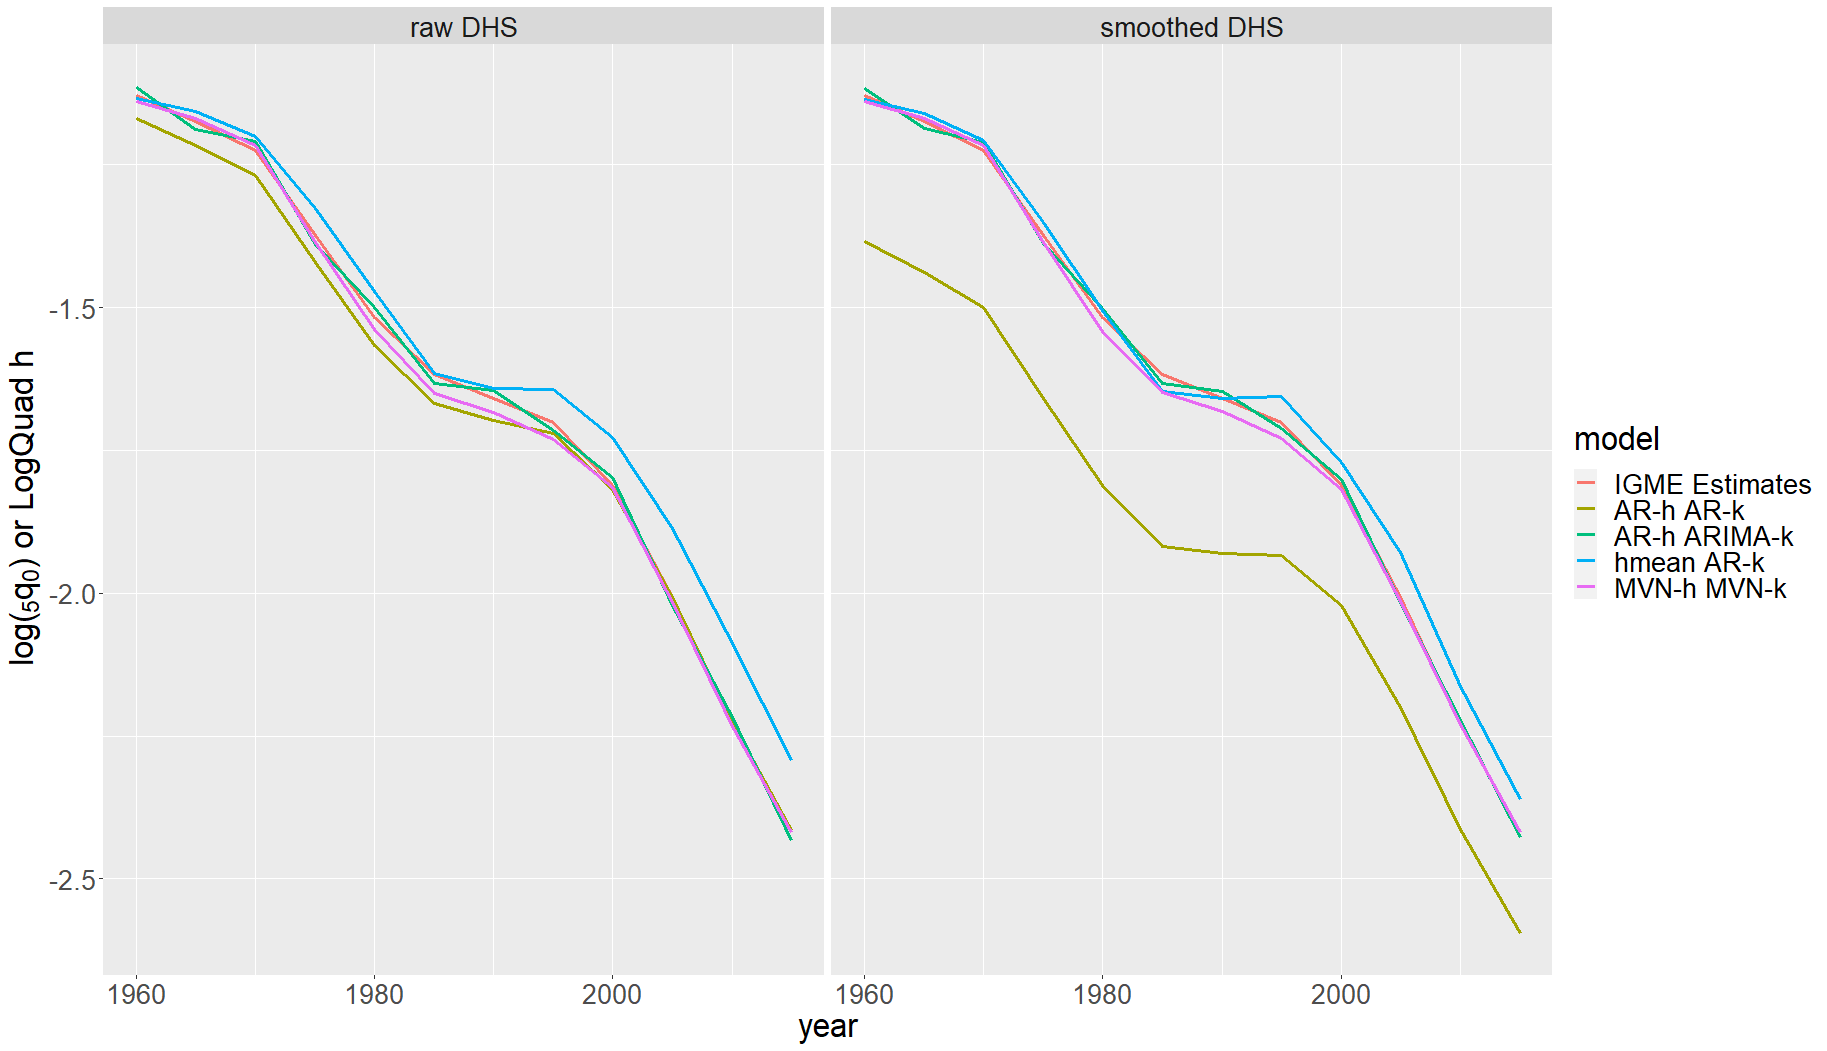
\includegraphics[width = \linewidth]{Burkina Faso/7/female h.png}
\end{figure}
\begin{figure}[H]
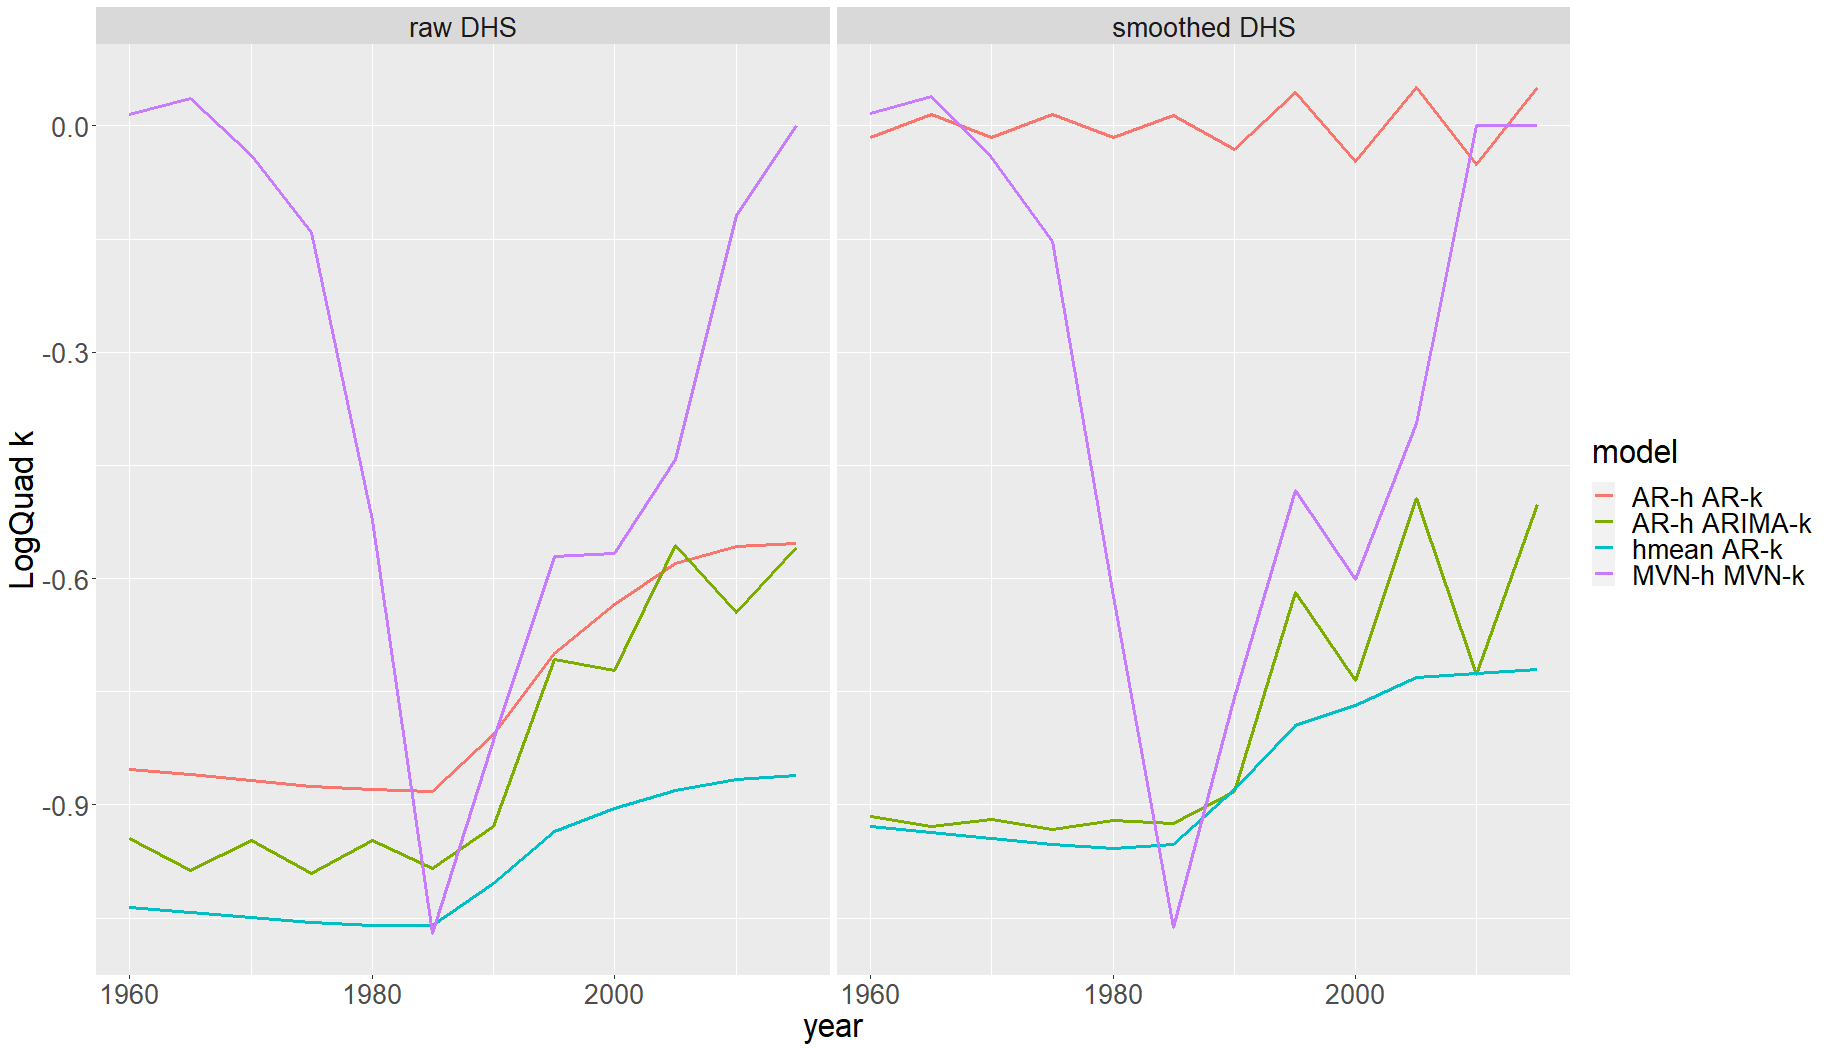
\includegraphics[width = \linewidth]{Burkina Faso/7/female k.png}
\end{figure}

\newpage
\section*{\centering Females only}
\begin{figure}[H]
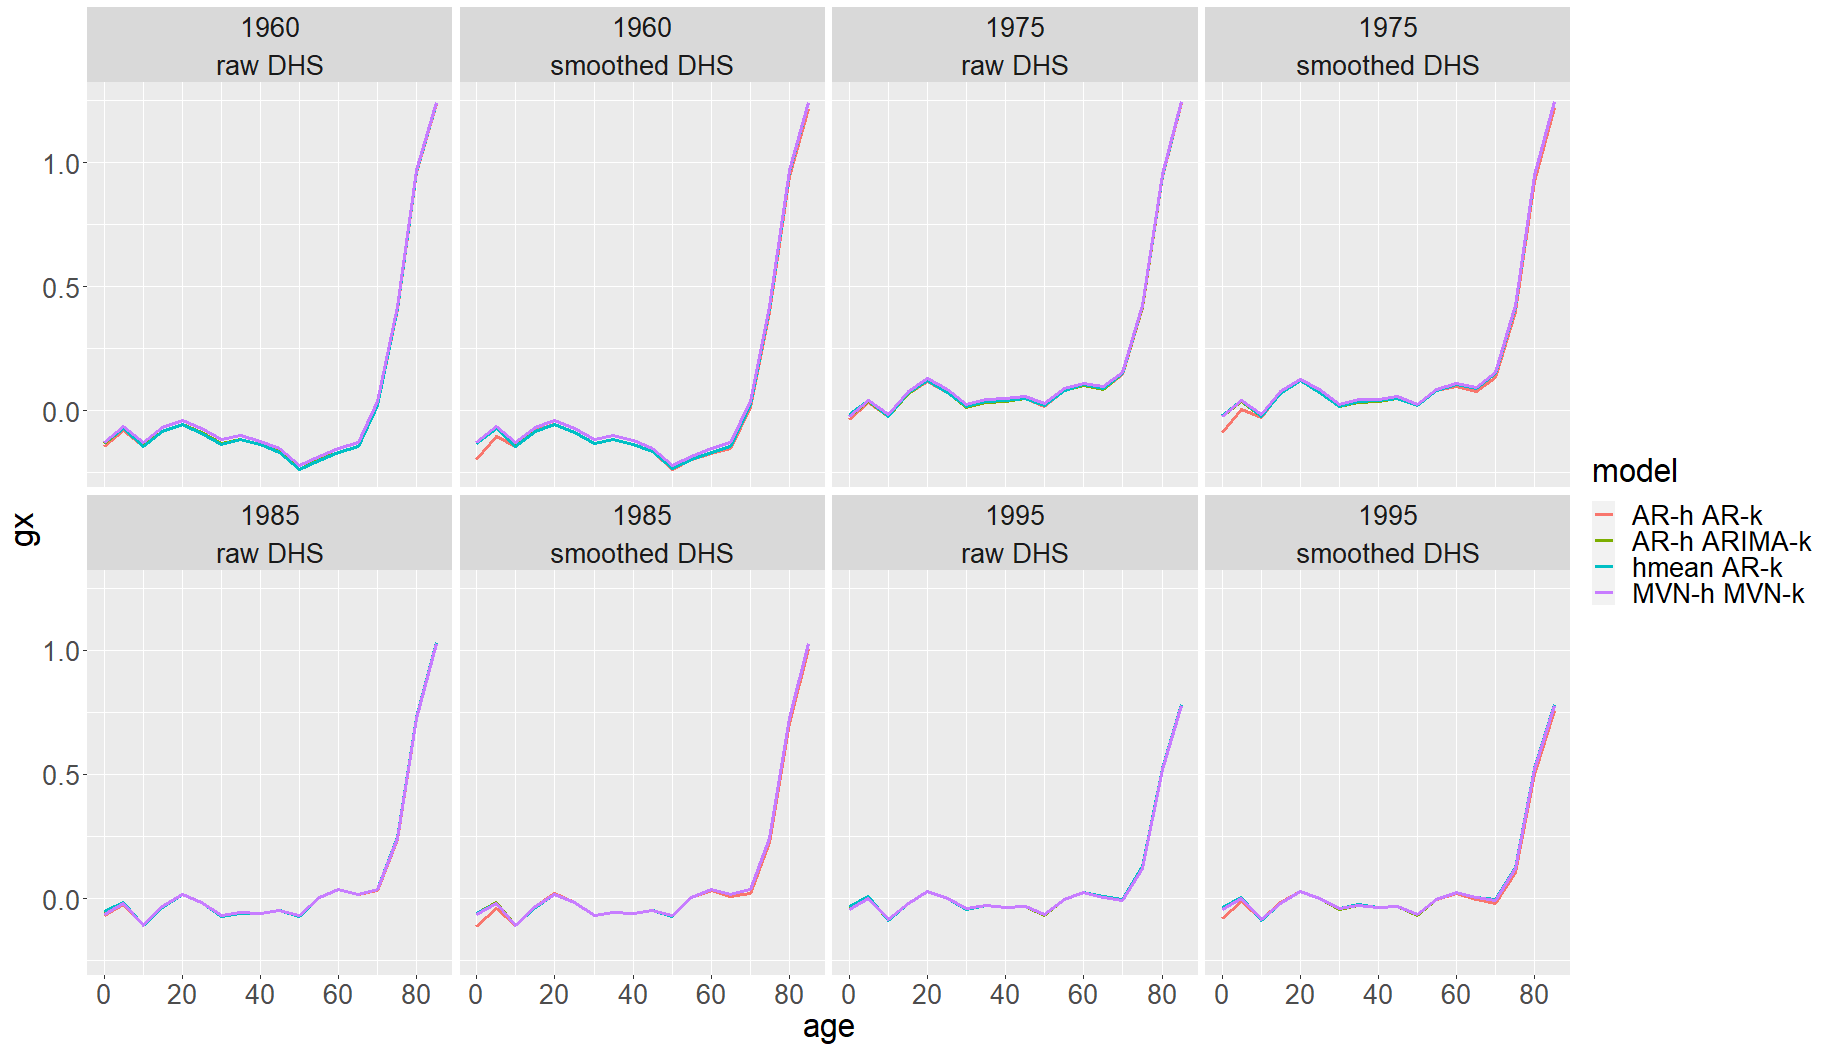
\includegraphics[width = \linewidth]{Burkina Faso/7/female mig.png}
\end{figure}
\begin{figure}[H]
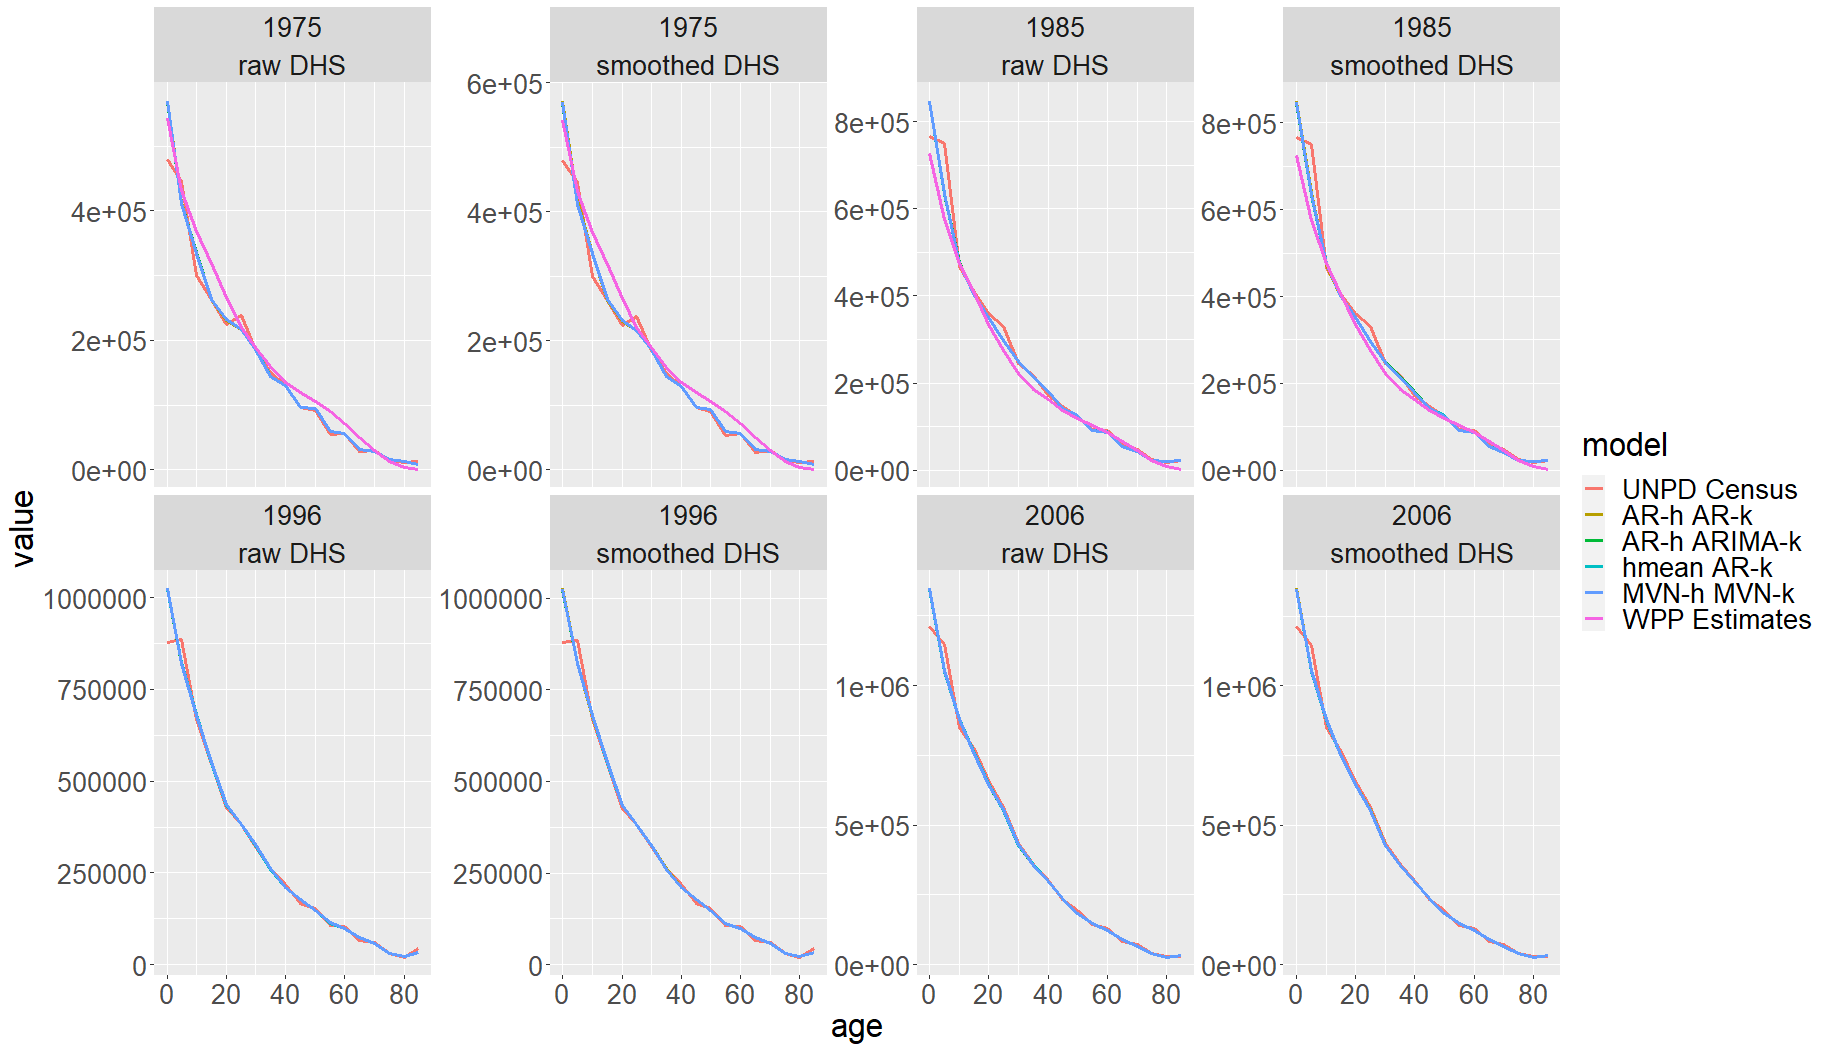
\includegraphics[width = \linewidth]{Burkina Faso/7/female period pop.png}
\end{figure}

\newpage
\section*{\centering Males only}
\begin{figure}[H]
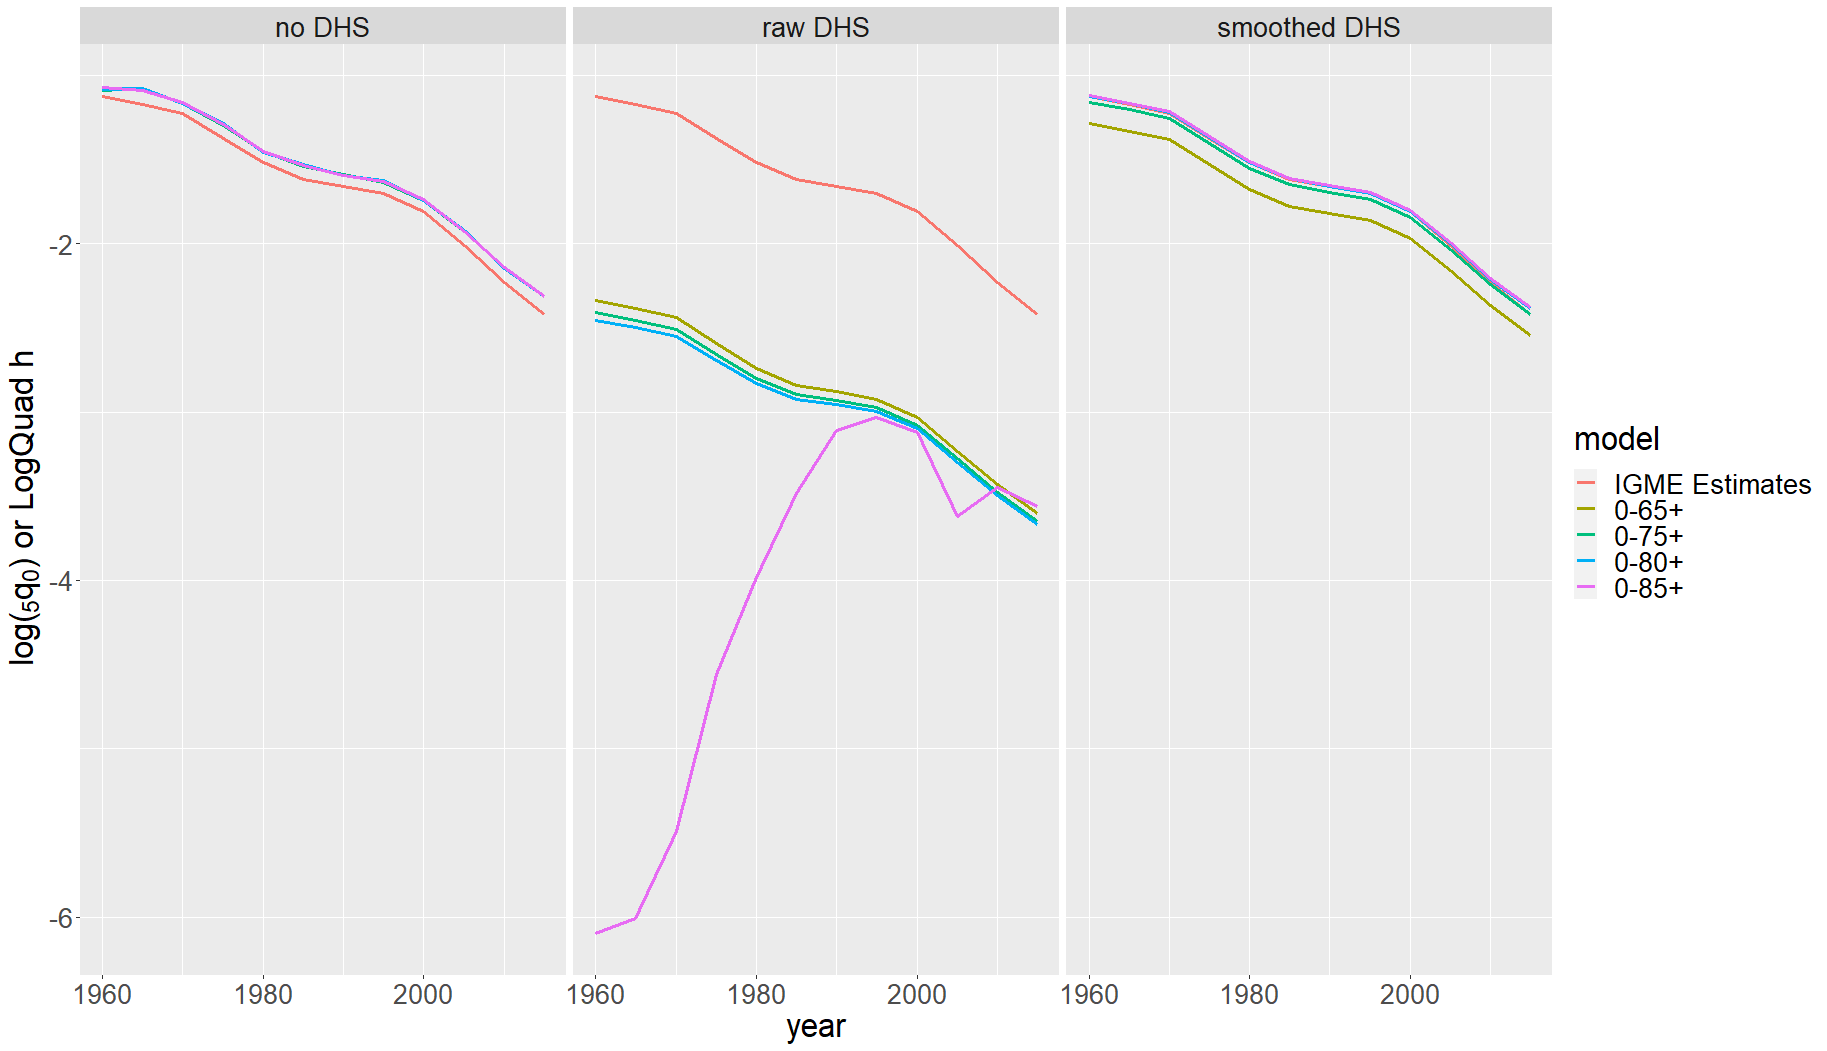
\includegraphics[width = \linewidth]{Burkina Faso/7/male h.png}
\end{figure}
\begin{figure}[H]
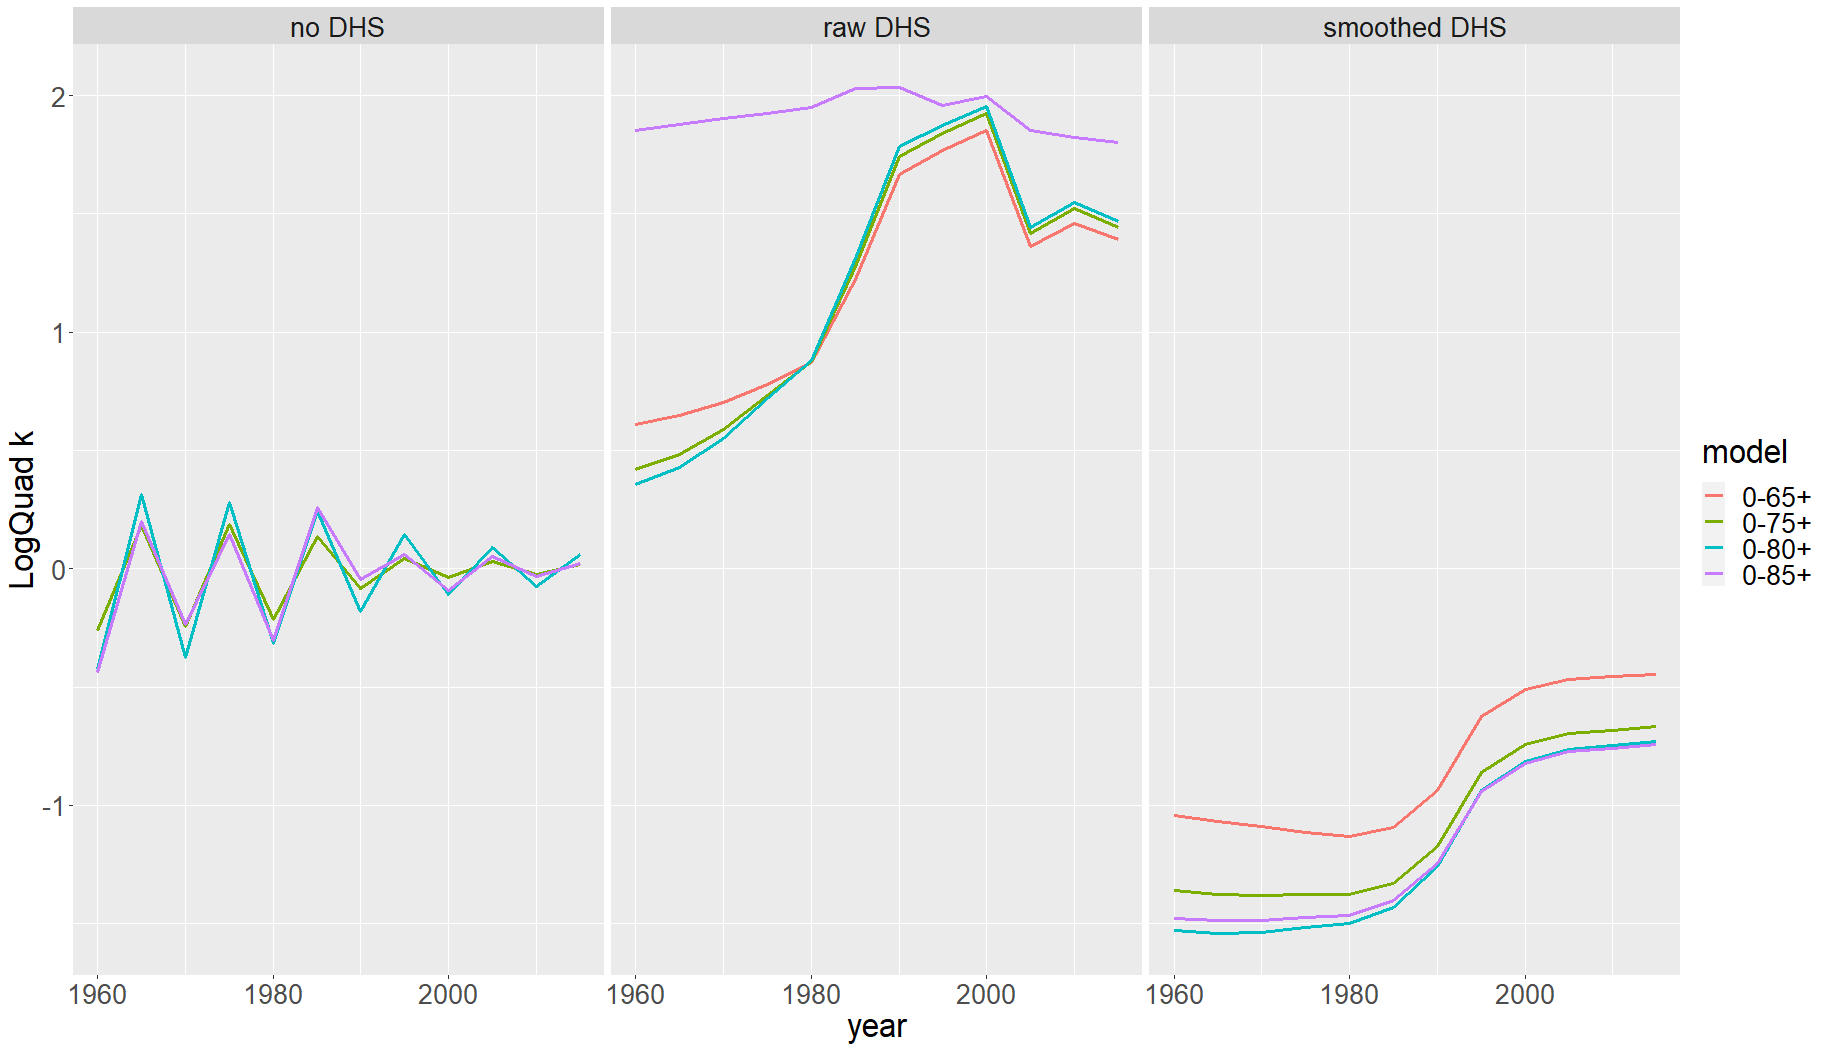
\includegraphics[width = \linewidth]{Burkina Faso/7/male k.png}
\end{figure}

\newpage
\section*{\centering Joint sex}
\begin{figure}[H]
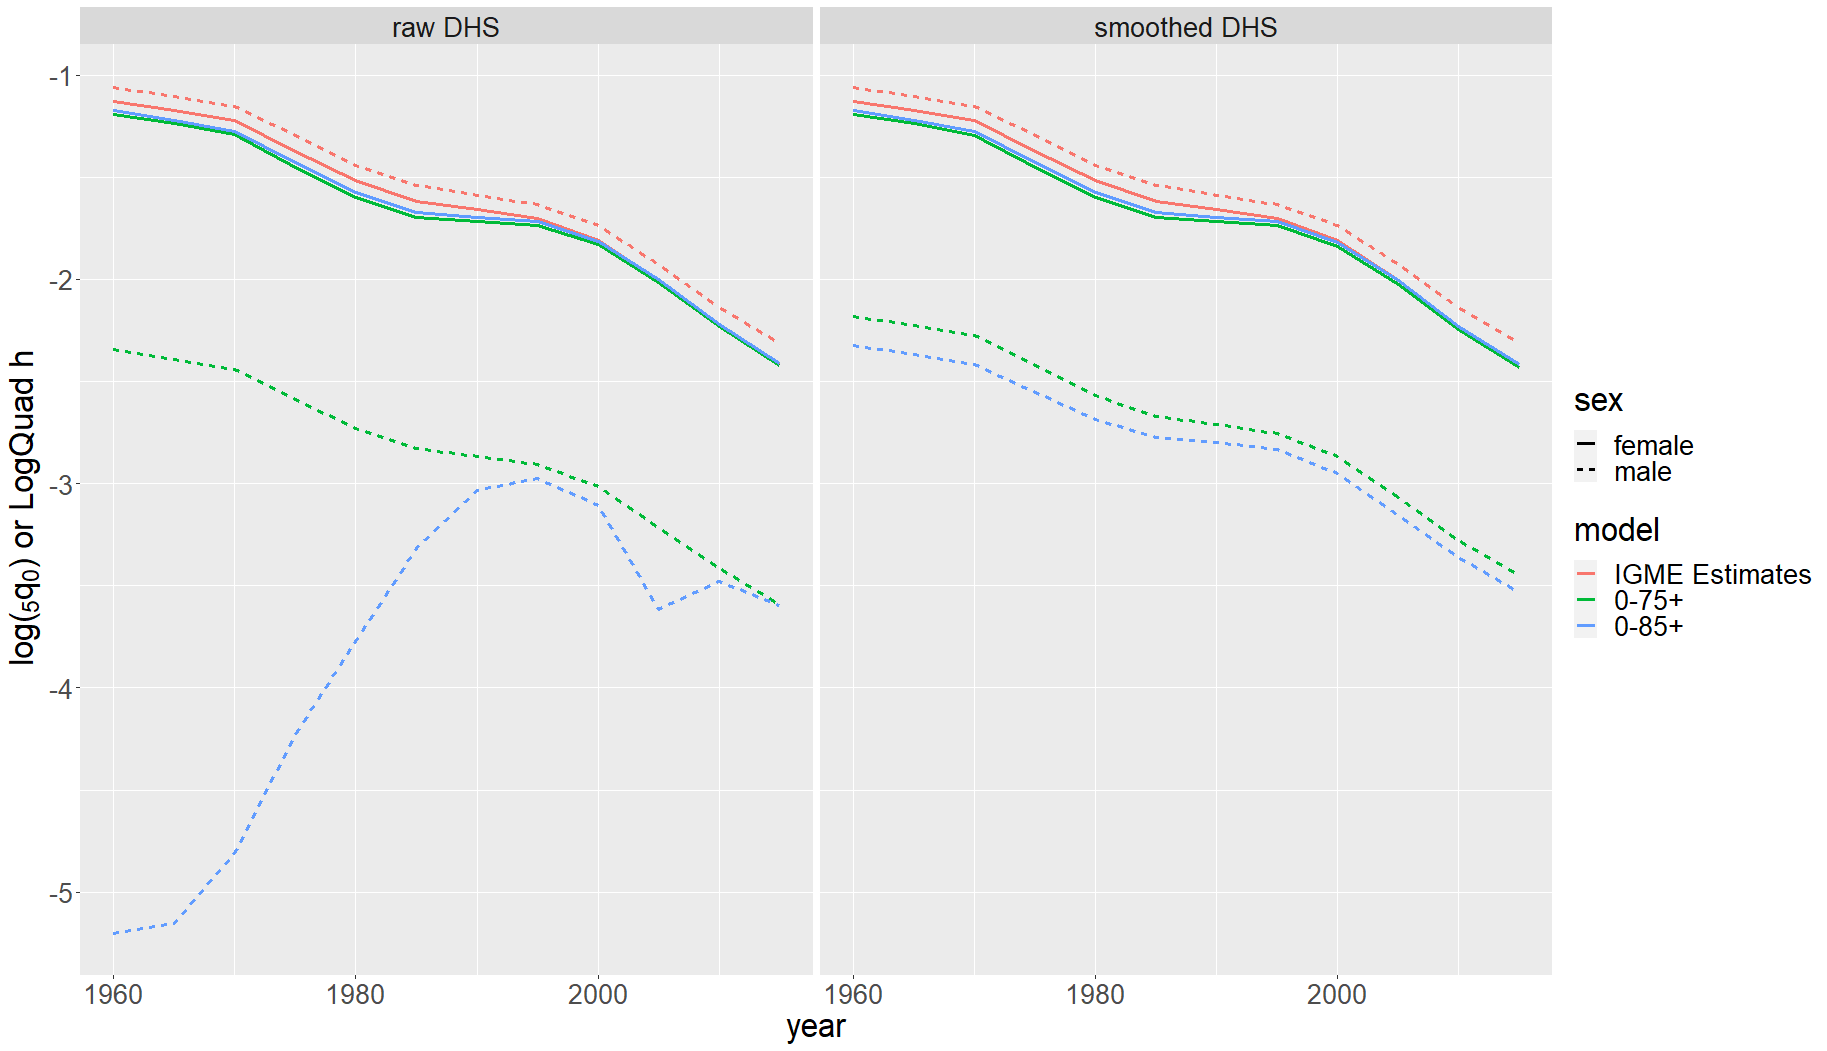
\includegraphics[width = \linewidth]{Burkina Faso/7/joint h.png}
\end{figure}
\begin{figure}[H]
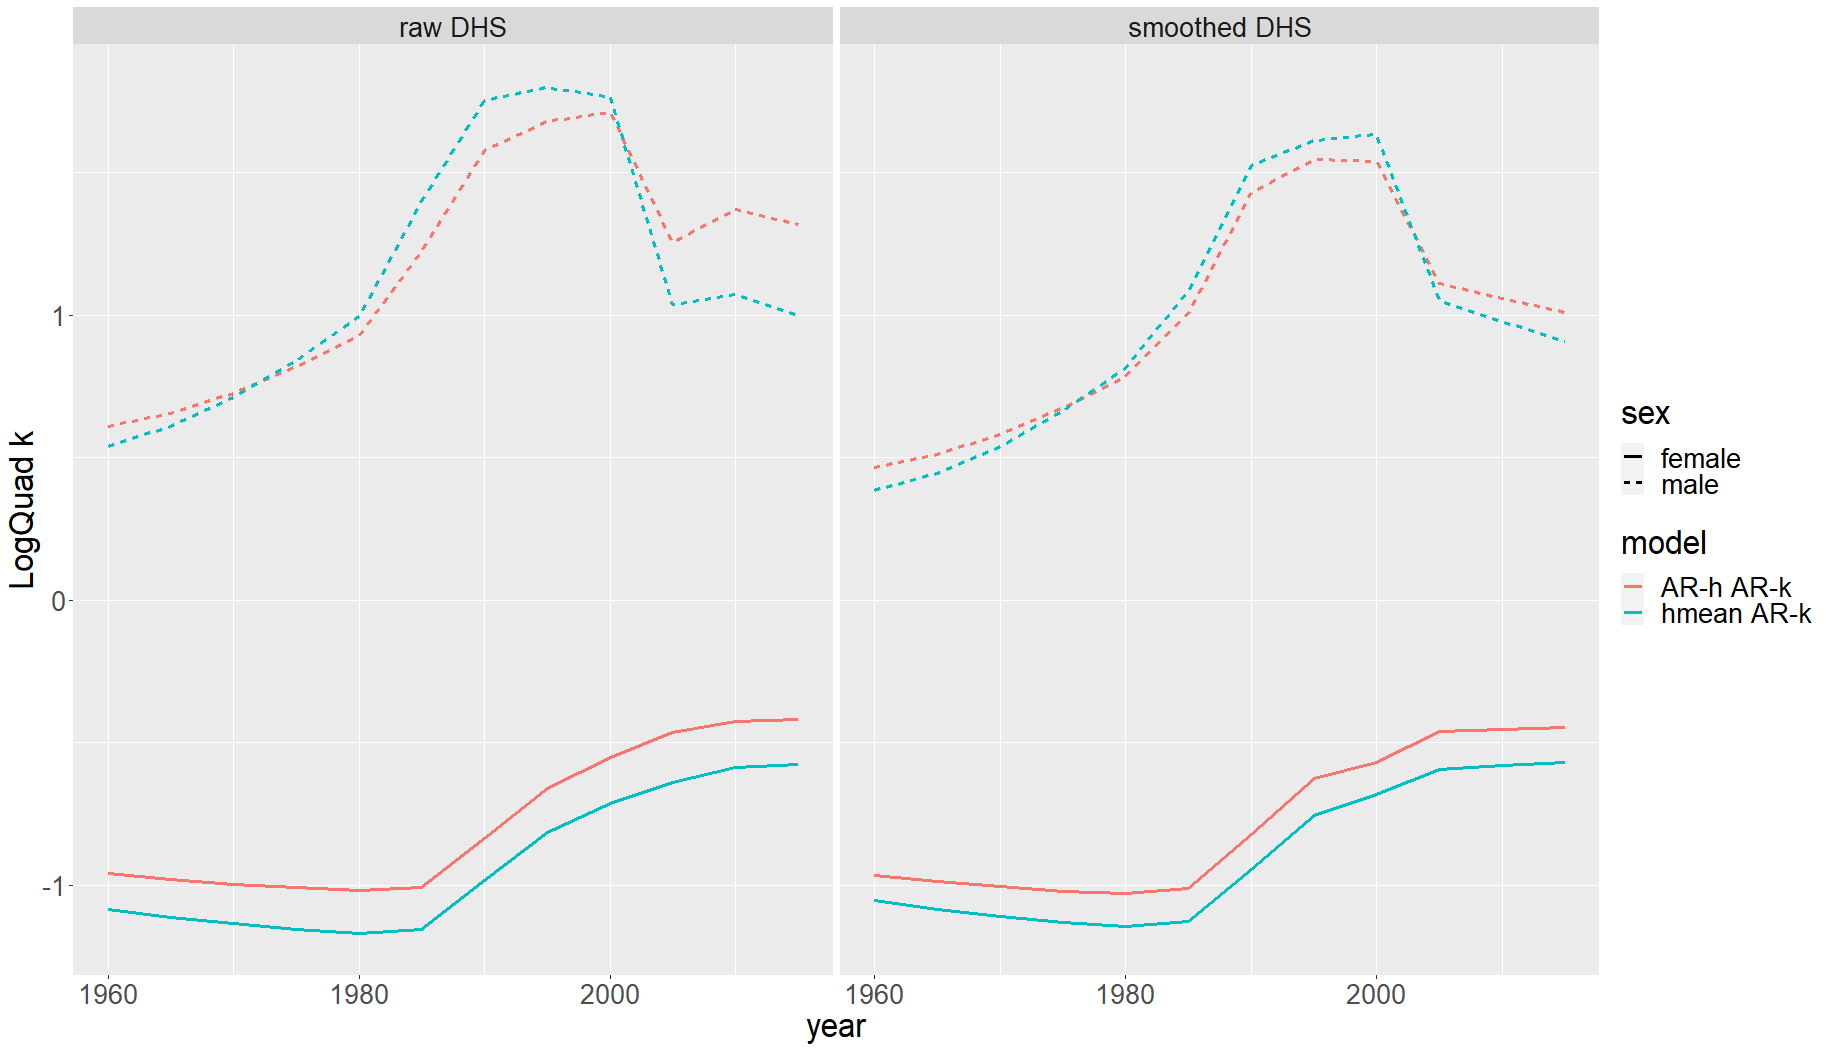
\includegraphics[width = \linewidth]{Burkina Faso/7/joint k.png}
\end{figure}

\newpage
\section*{\centering Joint sex}
\begin{figure}[H]
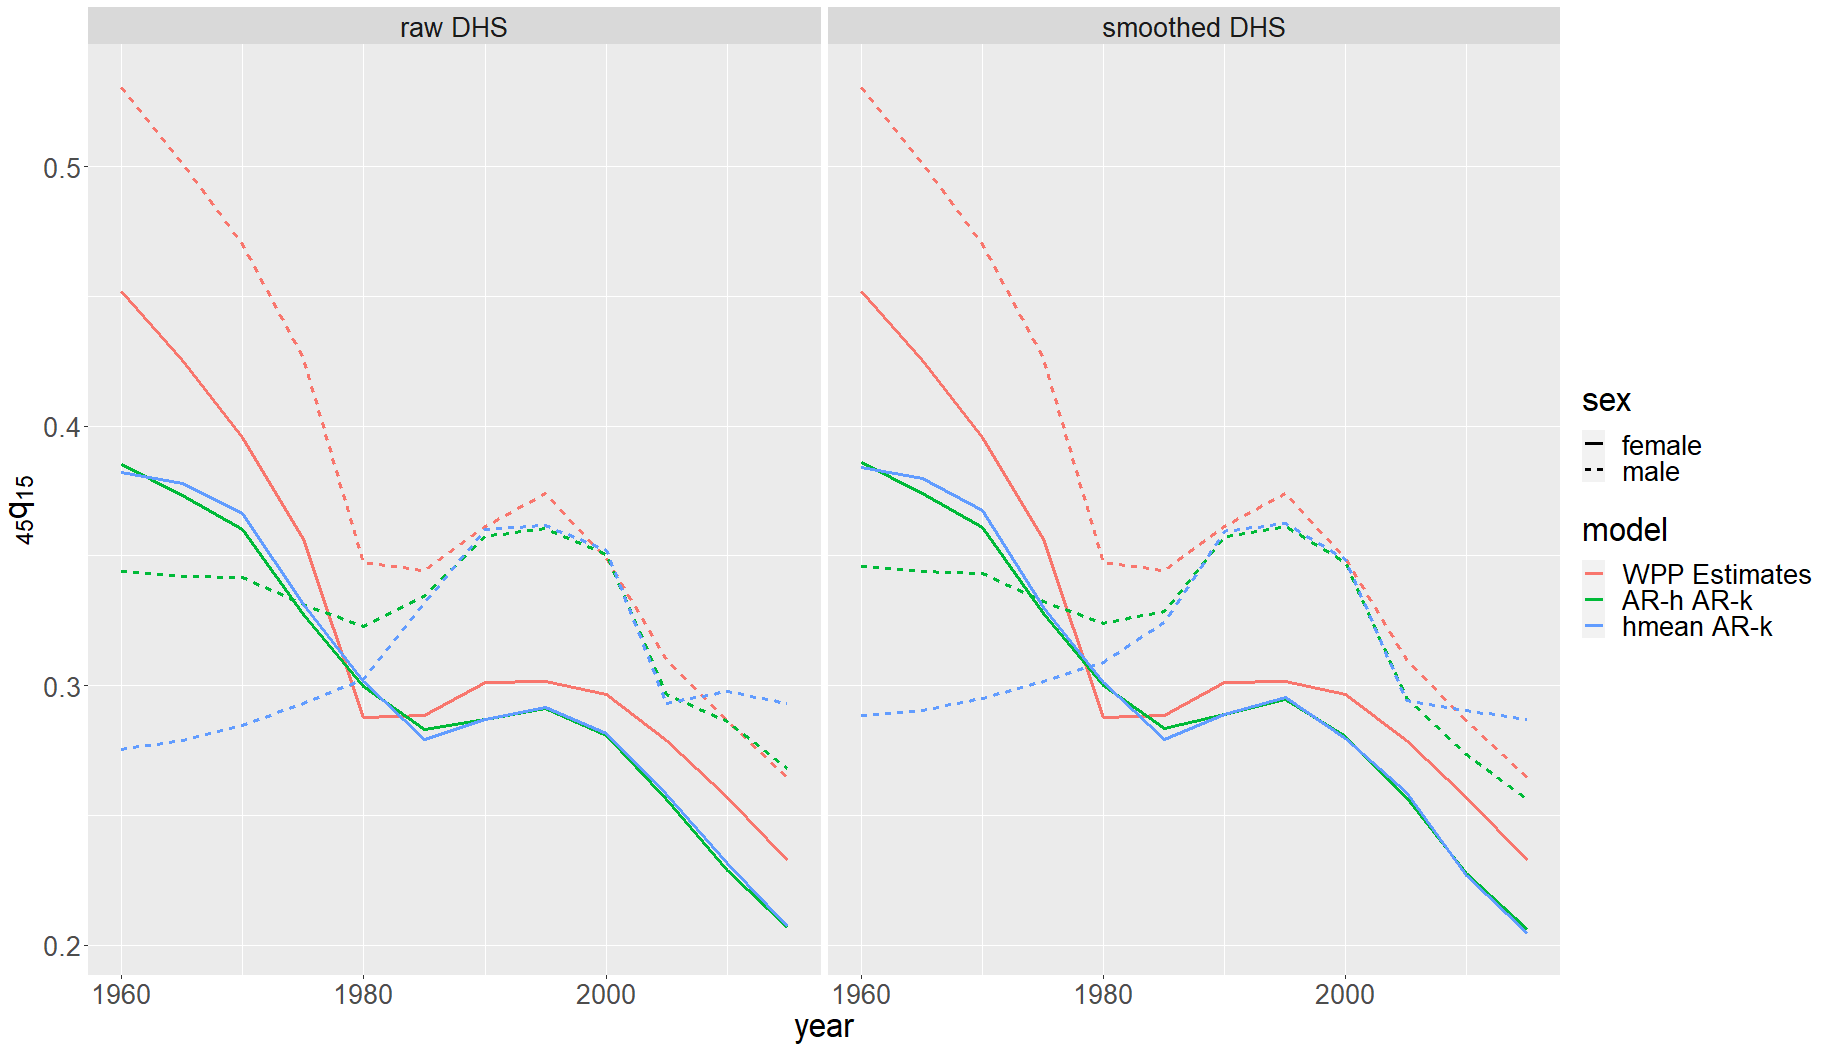
\includegraphics[width = \linewidth]{Burkina Faso/7/joint q4515.png}
\end{figure}
\begin{figure}[H]
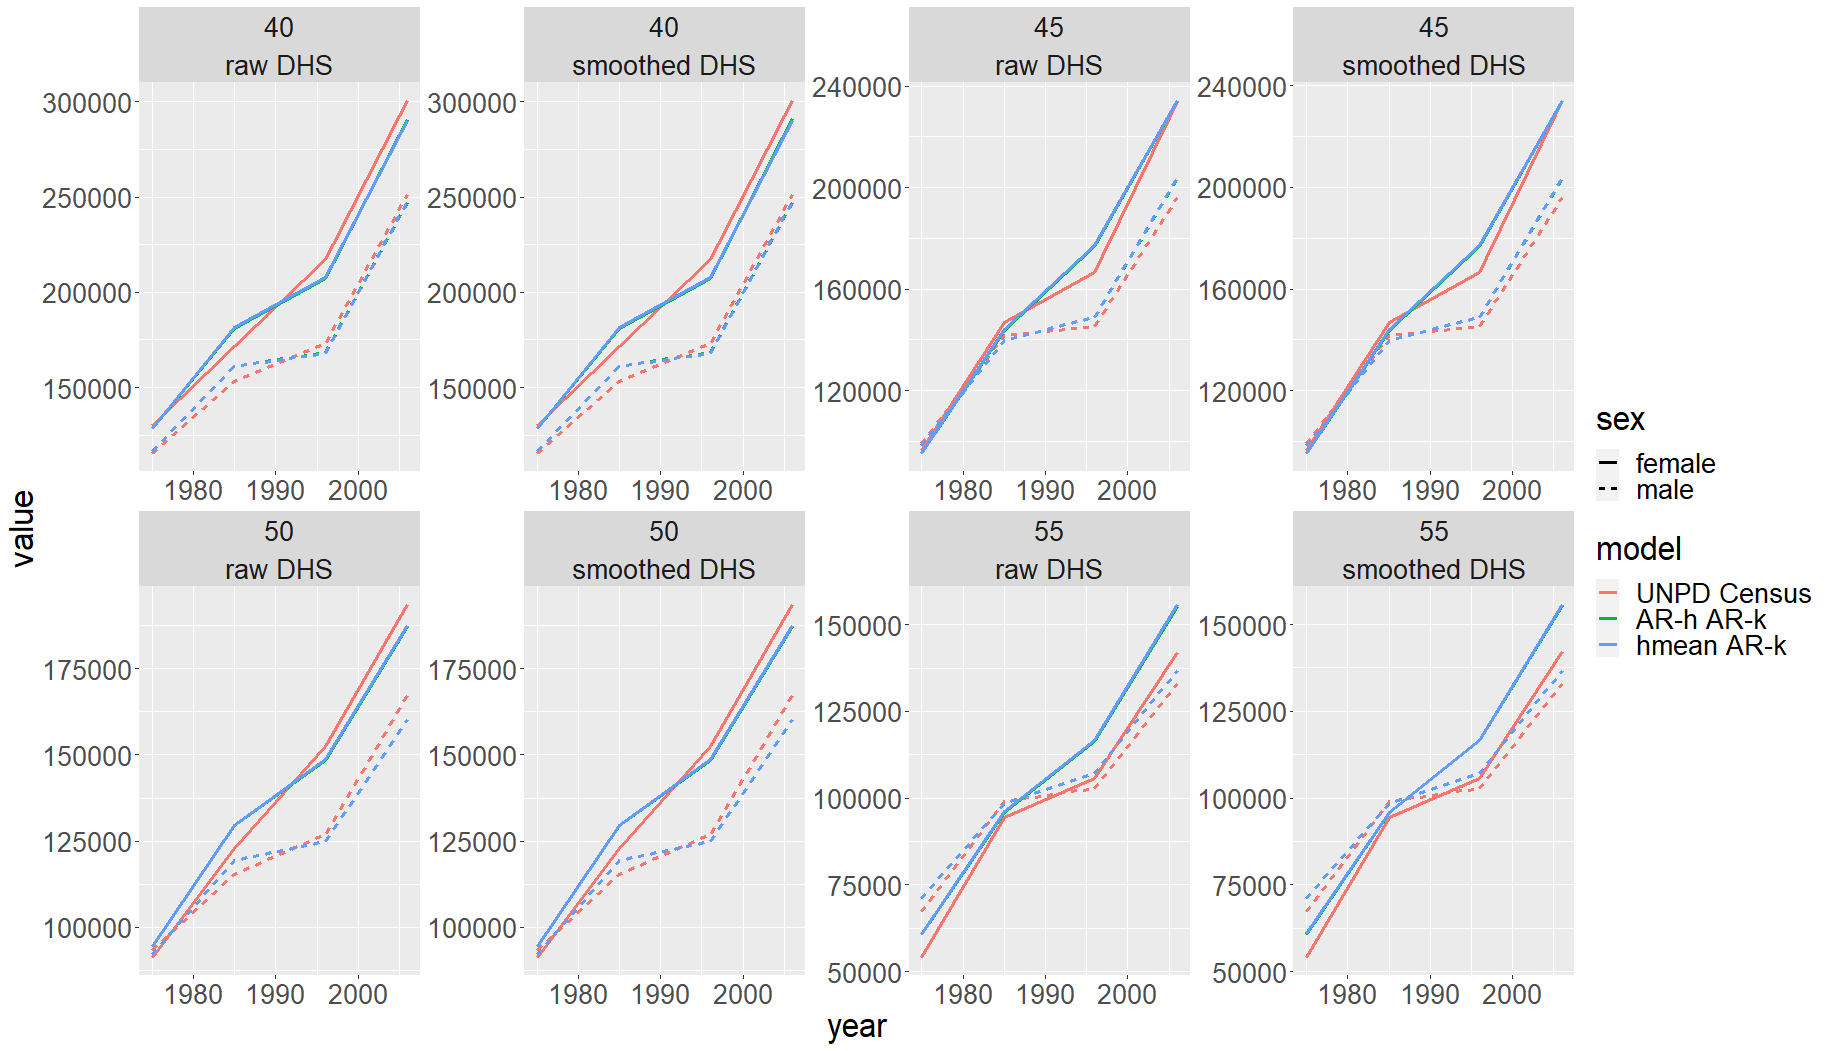
\includegraphics[width = \linewidth]{Burkina Faso/7/joint age pop.png}
\end{figure}

\section*{\centering Joint sex}
\begin{figure}[H]
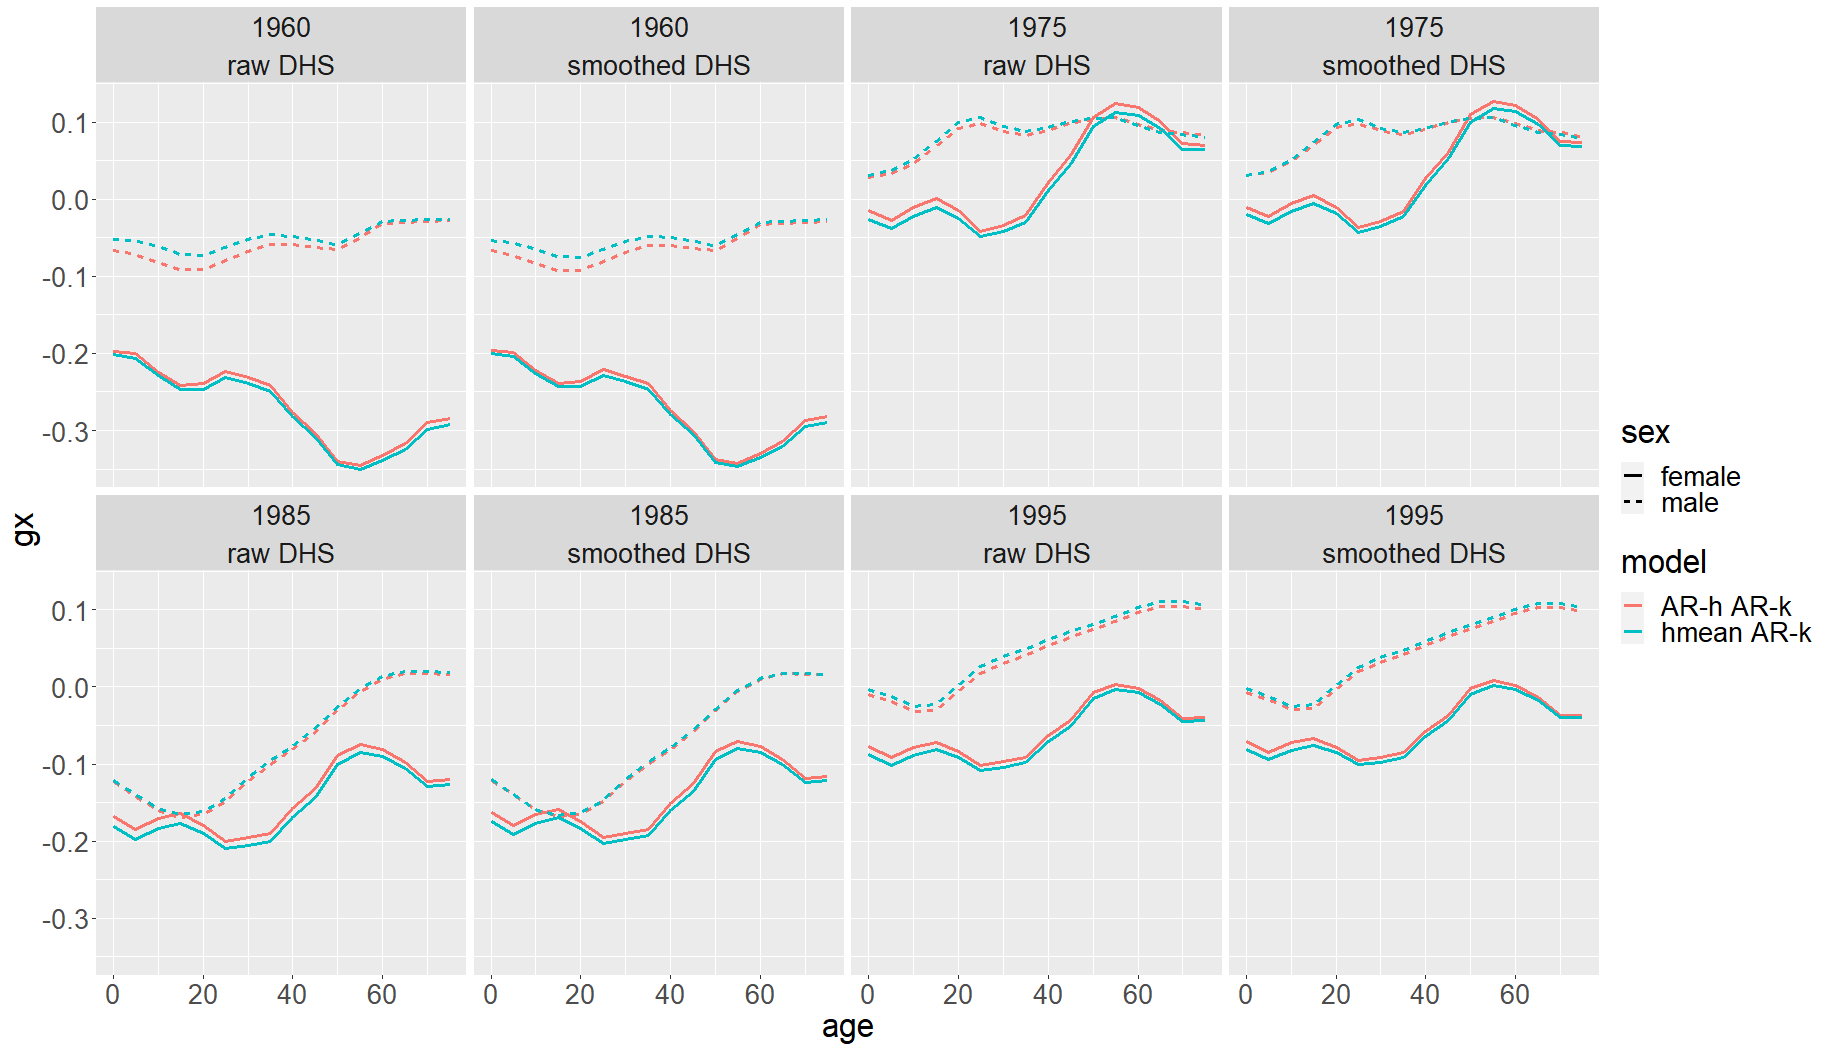
\includegraphics[width = \linewidth]{Burkina Faso/7/joint period mig.png}
\end{figure}
\begin{figure}[H]
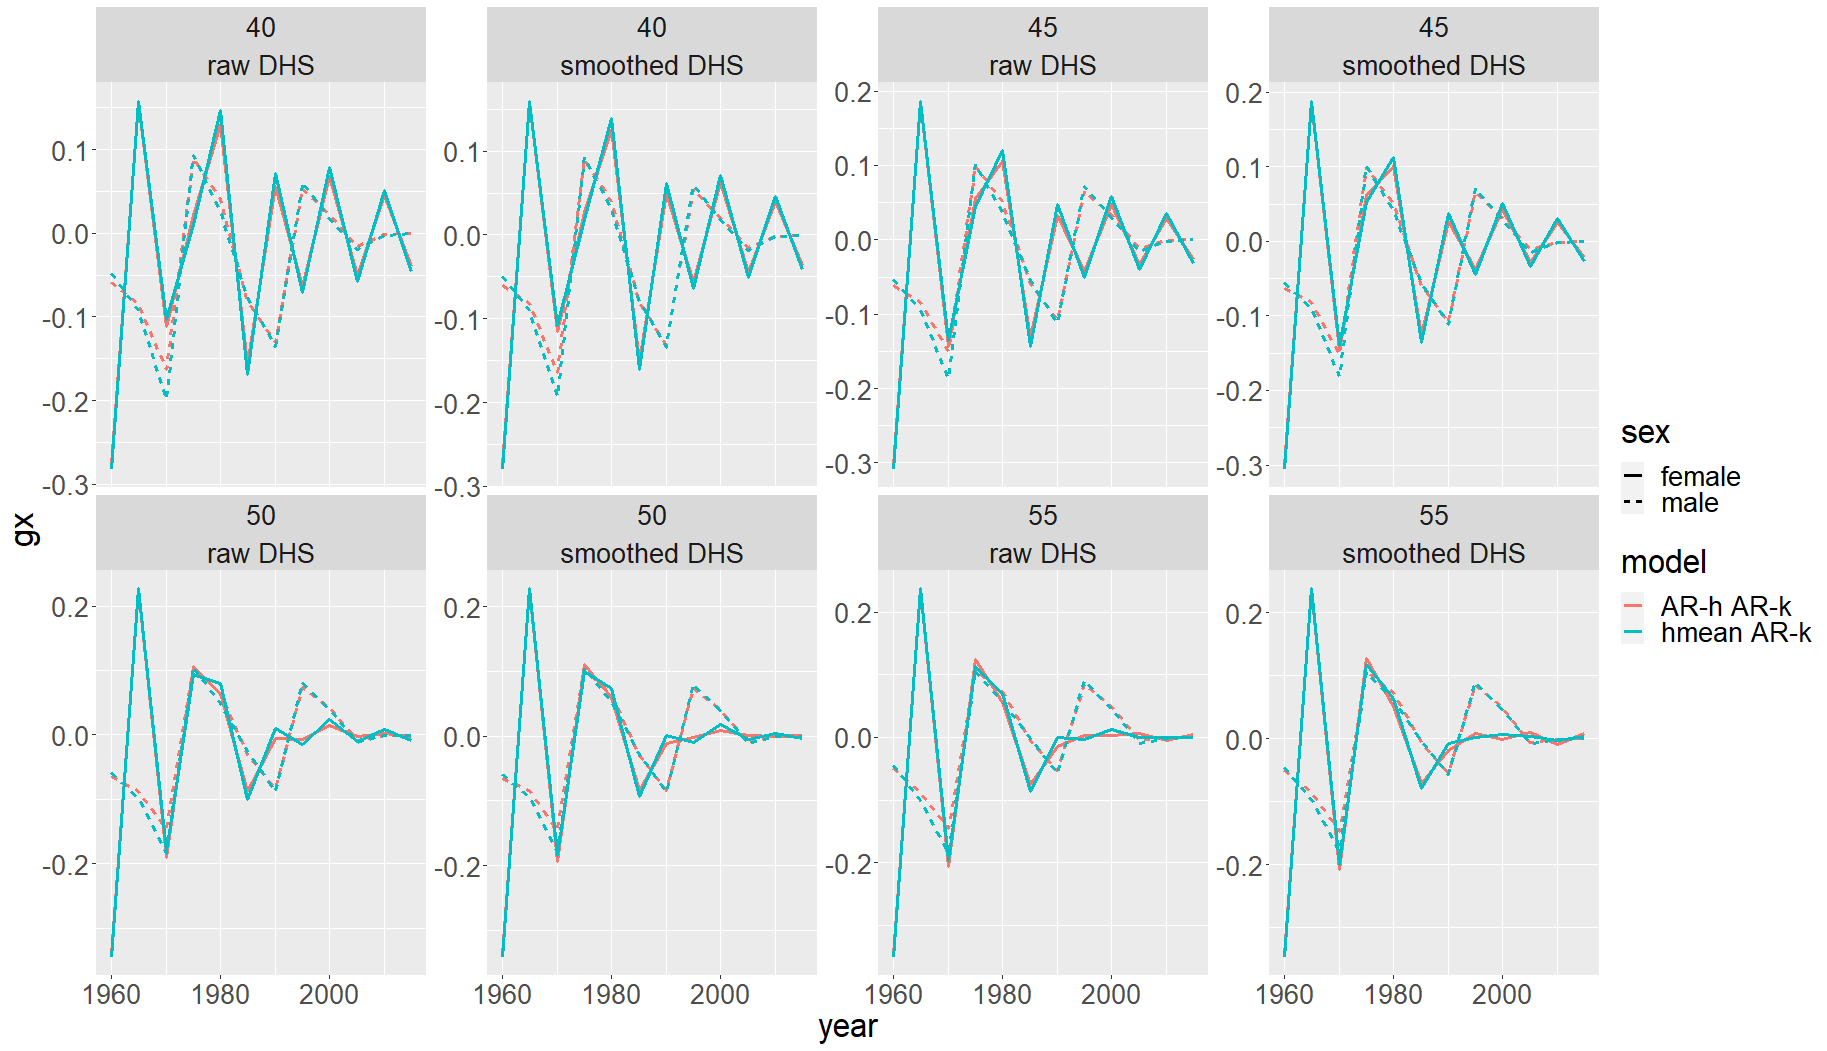
\includegraphics[width = \linewidth]{Burkina Faso/7/joint age mig.png}
\end{figure}


\newpage
\section*{\centering Joint sex}
\begin{figure}[H]
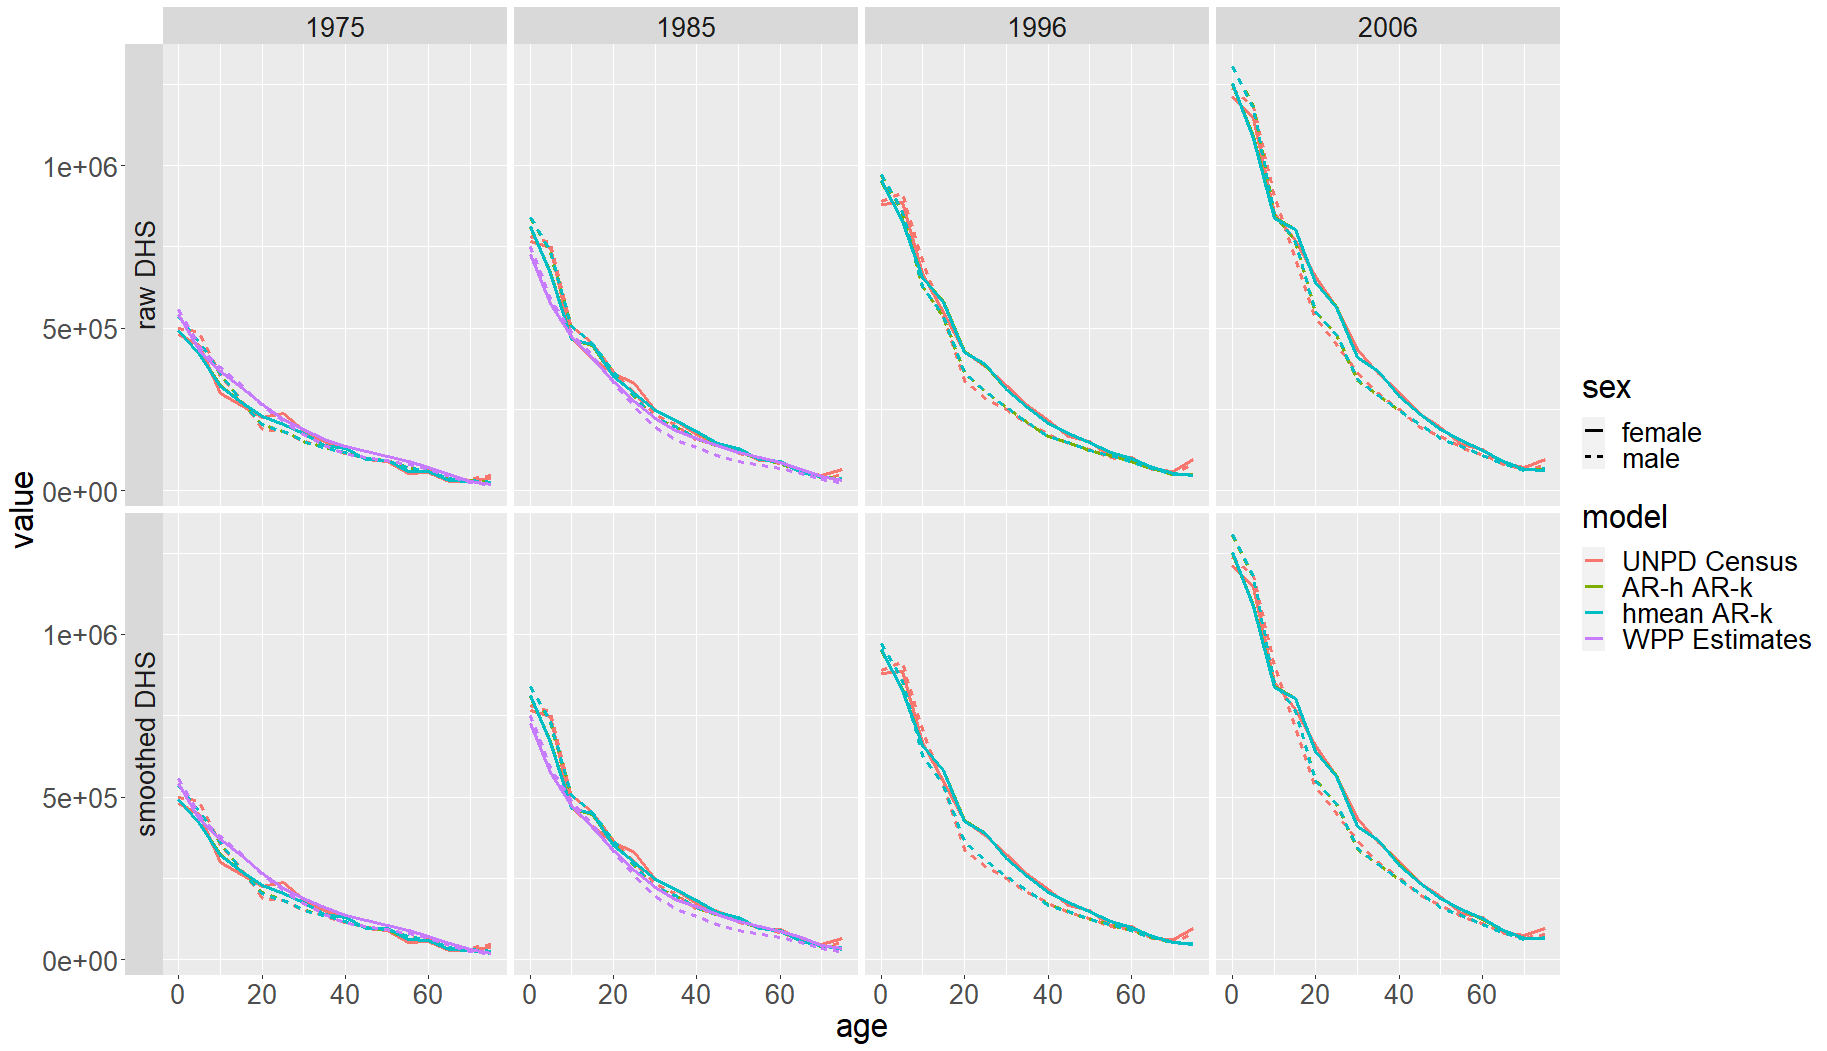
\includegraphics[width = \linewidth]{Burkina Faso/7/joint period pop.png}
\end{figure}
\begin{figure}[H]
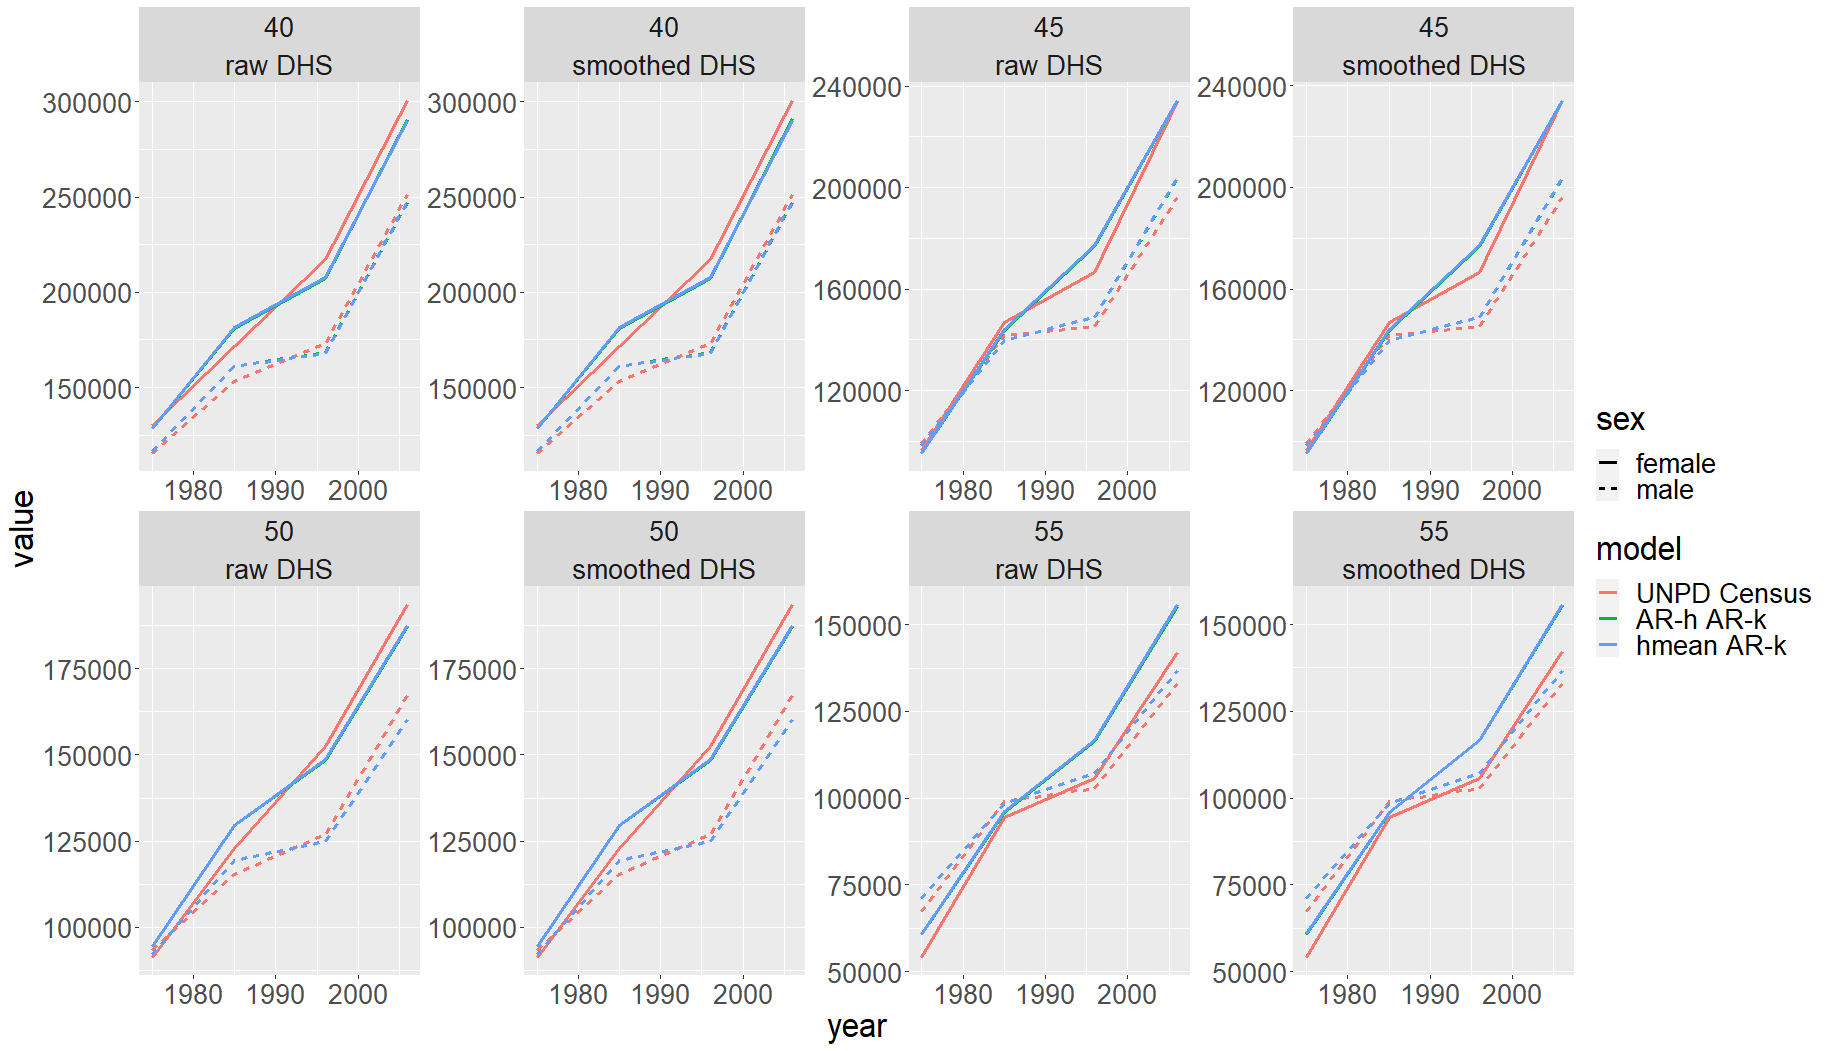
\includegraphics[width = \linewidth]{Burkina Faso/7/joint age pop.png}
\end{figure}


\end{document} 